%!TEX root=../GaugeCNNTheory.tex


\subsection{هندسه‌ی سطوح جایگذاری‌شده}
\label{sec:surfaces_geom_main}

این بخش یک مقدمه کوتاه بر هندسه سطوح ارائه می‌دهد.
برخی مفاهیم هندسه دیفرانسیل سطوح جایگذاری شده \emph{هموار} در بخش~\ref{sec:surfaces_geom_classical_smooth} مورد بحث قرار می‌گیرند.
بخش~\ref{sec:surfaces_geom_mesh} تلاش می‌کند تا یک نمای کلی از راه‌های ممکن برای \emph{گسسته‌سازی} کمیت‌های دیفرانسیل روی مش‌های سطحی ارائه دهد.

برای یک بررسی عمیق‌تر از سطوح پارامتری شده، خواننده را به \cite{gallier2011geomMethods} ارجاع می‌دهیم.
یک مقدمه مختصر و شهودی بر این موضوع و ارتباط آن با هندسه محاسباتی (گسسته‌سازی شده) را می‌توان در~\cite{craneDiscreteDifferentialGeometry2014} یافت.






\subsubsection{هندسه‌ی دیفرانسیل کلاسیک سطوح جایگذاری‌شده}
\label{sec:surfaces_geom_classical_smooth}

به طور کلاسیک، سطوح به صورت \emph{خارجی} توصیف شده‌اند، یعنی به عنوان غوطه‌ور (یا جایگذاری شده) در یک فضای محیطی اقلیدسی $\R^3$.
این غوطه‌وری را می‌توان به چندین روش معادل تعریف کرد، به عنوان مثال پارامتری‌سازی‌های محلی، وصله‌های مونژ یا توابع ضمنی.
پارامتری‌سازی‌های محلی سطح، نگاشت‌های همواری هستند
\begin{align}
    \chi:\, \R^2 \supset V \to M \subset \R^3
\end{align}
که زیرمجموعه‌های باز $V$ از $\R^2$ را در فضای محیطی $\R^3$ غوطه‌ور می‌کنند.
اینها باید منظم باشند، یعنی مشتقات جزئی آنها
\begin{align}
    e_i = \frac{\partial\chi}{\partial x_i}\ ,\qquad i=1,2
\end{align}
باید در $\R^3$ مستقل خطی باشند.
مشتقات $e_1(x_1,x_2) \in\R^3$ و $e_2(x_1,x_2) \in\R^3$
فضاهای مماس جایگذاری شده $\TpM \subset \R^3$ را در $p=\chi(x_1,x_2)$ تولید می‌کنند.%
\footnote{
    بردارهای مشتق $e_i$ در فرمالیسم چارت ذاتی با \emph{پایه‌های مختصاتی} مطابقت دارند؛ به پیوست~\ref{apx:coord_basis_def} مراجعه کنید.
}
بنابراین نرمال‌های سطح در فضای جایگذاری به خوبی تعریف شده و با $n = \frac{e_1 \times e_2}{\lVert e_1\times e_2\rVert}$ داده می‌شوند.
یک اطلس از پارامتری‌سازی‌های محلی سطح سازگار، امکان توصیف سطوحی را فراهم می‌کند که از نظر توپولوژیکی با صفحه در سطح جهانی متفاوت هستند.


متریک ریمانی سطح -- که در این زمینه اغلب به عنوان \emph{فرم بنیادی اول} آن شناخته می‌شود -- از فضای جایگذاری القا می‌شود.
مطابق با تعریف مشابه برای کره جایگذاری شده $S^2$ در معادله~\eqref{eq:spherical_embedding_metric_explicit} داریم:
\begin{align}\label{eq:surface_embedding_metric}
    \eta_p(v,w) \,:=\, \langle v,w \rangle_{\R^3} \qquad \forall\ v,w \in \TpM
\end{align}
فرض کنید $v = \sum_i \mathscr{v}_i e_i$ و $w = \sum_i \mathscr{w}_i e_i$ بردارهای مماس در $\TpM$ باشند که بر حسب بردارهای ضریب خود $\mathscr{v},\mathscr{w}\in\R^2$ نسبت به پایه مختصاتی بیان شده‌اند.
متریک نسبت به این پایه با یک ماتریس ضریب متقارن نمایش داده می‌شود
\begin{align}
    \operatorname{I}
    \ =\ 
    \begin{pmatrix}
        E \mkern-8mu& F \\
        F \mkern-8mu& G
    \end{pmatrix}
\end{align}
با درایه‌های%
\footnote{
    در نمادگذاری مدرن، ضرایب یک متریک (مستقل از مختصات) $g$ نسبت به یک پایه داده شده اغلب با $g_{\mu\nu}$ نشان داده می‌شوند.
}
$E = \langle e_1, e_1 \rangle_{\R^3}$,
$F = \langle e_1, e_2 \rangle_{\R^3}
    = \langle e_2, e_1 \rangle_{\R^3}$ و
$G = \langle e_2, e_2 \rangle_{\R^3}$.
این ماتریس بر روی ضرایب برداری مطابق با $\eta_p(v,w) = \mathscr{v}^\top \operatorname{I}\mathscr{w}$ عمل می‌کند.
فرم بنیادی اول، هندسه \emph{ذاتی} یک سطح را به عنوان یک منیفلد ریمانی دوبعدی کدگذاری می‌کند، یعنی آن بخشی از هندسه که مستقل از غوطه‌وری آن در فضای محیطی است.


هندسه \emph{خارجی} یک سطح، یعنی جزئیات مربوط به غوطه‌وری خاص آن در فضای محیطی، توسط \emph{فرم بنیادی دوم} آن ثبت می‌شود.
نسبت به $e_1$ و $e_2$ این فرم با ماتریس
\begin{align}
    \operatorname{I\!I}
    \ =\ 
    \begin{pmatrix}
        L \mkern-8mu& M \\
        M \mkern-8mu& N
    \end{pmatrix}
\end{align}
با درایه‌های
$L = \big\langle n, \frac{\partial^2\chi}{\partial x_1^2} \big\rangle_{\R^3}
    = \big\langle n, \frac{\partial e_1}{\partial x_1} \big\rangle_{\R^3}$,
$M = \big\langle n, \frac{\partial^2\chi}{\partial x_1 \partial x_2} \big\rangle_{\R^3}
    = \big\langle n, \frac{\partial e_1}{\partial x_2} \big\rangle_{\R^3}
    = \big\langle n, \frac{\partial e_2}{\partial x_1} \big\rangle_{\R^3}$
و
$N = \big\langle n, \frac{\partial^2\chi}{\partial x_2^2} \big\rangle_{\R^3}
    = \big\langle n, \frac{\partial e_2}{\partial x_2} \big\rangle_{\R^3}$ نمایش داده می‌شود.
این درایه‌ها اساساً اندازه‌گیری می‌کنند که پایه‌های مختصاتی -- و در نتیجه فضاهای مماس -- در فضای محیطی (در جهت نرمال) هنگام حرکت در امتداد خطوط مختصاتی چقدر خم می‌شوند.
این فرم را می‌توان به عنوان مثال برای تعیین \emph{انحنای نرمال}
\begin{align}
    \kappa_n(v)\ =\ \frac{\mathscr{v}^\top \operatorname{I\!I}\mathscr{v}}{\mathscr{v}^\top \operatorname{I}\mathscr{v}}
\end{align}
سطح در $p$ در جهت $v = \sum_i \mathscr{v}_i e_i \in \TpM$ استفاده کرد.
به طور شهودی، این انحنای نرمال را می‌توان به عنوان انحنای منحنی تعریف شده توسط تقاطع سطح با صفحه تولید شده توسط جهت $v$ و نرمال $n$ در آن نقطه درک کرد.
این انحنا با معکوس شعاع $r=1/\kappa_n(v)$ دایره بوسان بر منحنی در $p$ مطابقت دارد و بنابراین اندازه‌گیری می‌کند که سطح هنگام حرکت در جهت $v$ چقدر در جهت نرمال خم می‌شود؛ برای تجسم عالی این وضعیت به~\cite{craneDiscreteDifferentialGeometry2014} مراجعه کنید.
کمیت‌های مورد علاقه دیگر در مطالعه سطوح غوطه‌ور شده، انحناهای اصلی، میانگین و گاوسی آنها هستند که می‌توانند بر حسب انحناهای نرمال بیان شوند و در شکل~\ref{fig:curvature_surfaces} مثال زده شده‌اند.
جهت‌ها (بردارهای واحد در $\TpM$) $v_{\max}$ و $v_{\min}$ که در آنها انحنای نرمال در یک نقطه داده شده $p$ حداکثر یا حداقل است، به عنوان \emph{جهات اصلی} در~$p$ شناخته می‌شوند.
انحناهای متناظر
\begin{align}
    \kappa_{\max} = \kappa_n(v_{\max})
    \qquad \textup{and} \qquad
    \kappa_{\min} = \kappa_n(v_{\min})
\end{align}
\emph{انحناهای اصلی} در~$p$ هستند.
مقدار میانگین آنها
\begin{align}\label{eq:mean_curvature}
    \kappa_{\textup{mean}} \ =\ \frac{\kappa_{\max}+\kappa_{\min}}{2}
\end{align}
به عنوان \emph{انحنای میانگین} شناخته می‌شود.
انحنای میانگین در نقاط «زین‌مانند» که $\kappa_{\min} = -\kappa_{\max}$ است، صفر است.
سطوح کمینه در هر نقطه انحنای میانگین صفر دارند.
حاصلضرب
\begin{align}
    \kappa_{\textup{Gauss}}\ =\ \kappa_{\max} \cdot \kappa_{\min}
\end{align}
انحناهای اصلی به عنوان \emph{انحنای گاوسی} شناخته می‌شود.
این انحنا مثبت است اگر انحناهای اصلی هم‌علامت باشند، که به عنوان مثال برای بیضی‌گون‌ها صادق است.
برای اینکه انحنای گاوسی منفی باشد، علامت انحناهای اصلی باید متفاوت باشد، مانند اطراف نواحی هذلولی (زین‌مانند).
انحنای گاوسی صفر است اگر یکی (یا هر دو) از مقادیر انحنای اصلی صفر باشد، یعنی اگر سطح یک جهت تخت داشته باشد.
یک مثال برای یک منیفلد با انحنای گاوسی صفر، استوانه است.
گفته می‌شود چنین سطوحی \emph{گسترش‌پذیر} هستند، که به این معنی است که می‌توان آنها را بدون تغییر شکل به یک صفحه پهن کرد، یا به طور دقیق‌تر، آنها به صورت محلی با صفحه ایزومتریک هستند.
کارل فریدریش گاوس در \emph{قضیه شگفت‌انگیز} خود اثبات کرد که انحنای گاوسی یک سطح در واقع یک ویژگی ذاتی است، یعنی به نحوه غوطه‌وری سطح در فضای محیطی بستگی ندارد.
این انحنا در تناظر یک به یک با تانسور انحنای ریمانی (ذاتی) یک سطح است (و بنابراین با انحنای ریچی و اسکالر آن نیز).
یک ویژگی مهم انحنای گاوسی این است که انتگرال آن روی یک دیسک توپولوژیکی $D \subset M$ برابر با هولونومی $\delta_{\partial\mkern-1mu D}$ است، یعنی زاویه‌ای که یک بردار هنگام انتقال (لوی-چیویتا) یک بار حول مرز دیسک~$\partial\mkern-1mu D$ می‌چرخد:
\begin{align}\label{eq:gauss_curvature_holonomy_smooth}
    \int_{D} \kappa_{\textup{Gauss}}\, dp\ =\ \delta_{\partial\mkern-1mu D}
\end{align}
همانطور که در ادامه خواهیم دید، این رابطه را می‌توان برای تعمیم انحنای گاوسی به مش‌ها استفاده کرد، جایی که هولونومی $\delta_{\partial\mkern-1mu D}$ با نقص زاویه یک حلقه باز شده از وجوه (مانند همسایگی آبی در شکل~\ref{fig:ico_neighborhoods}) مطابقت دارد.

\begin{figure}
    \centering
    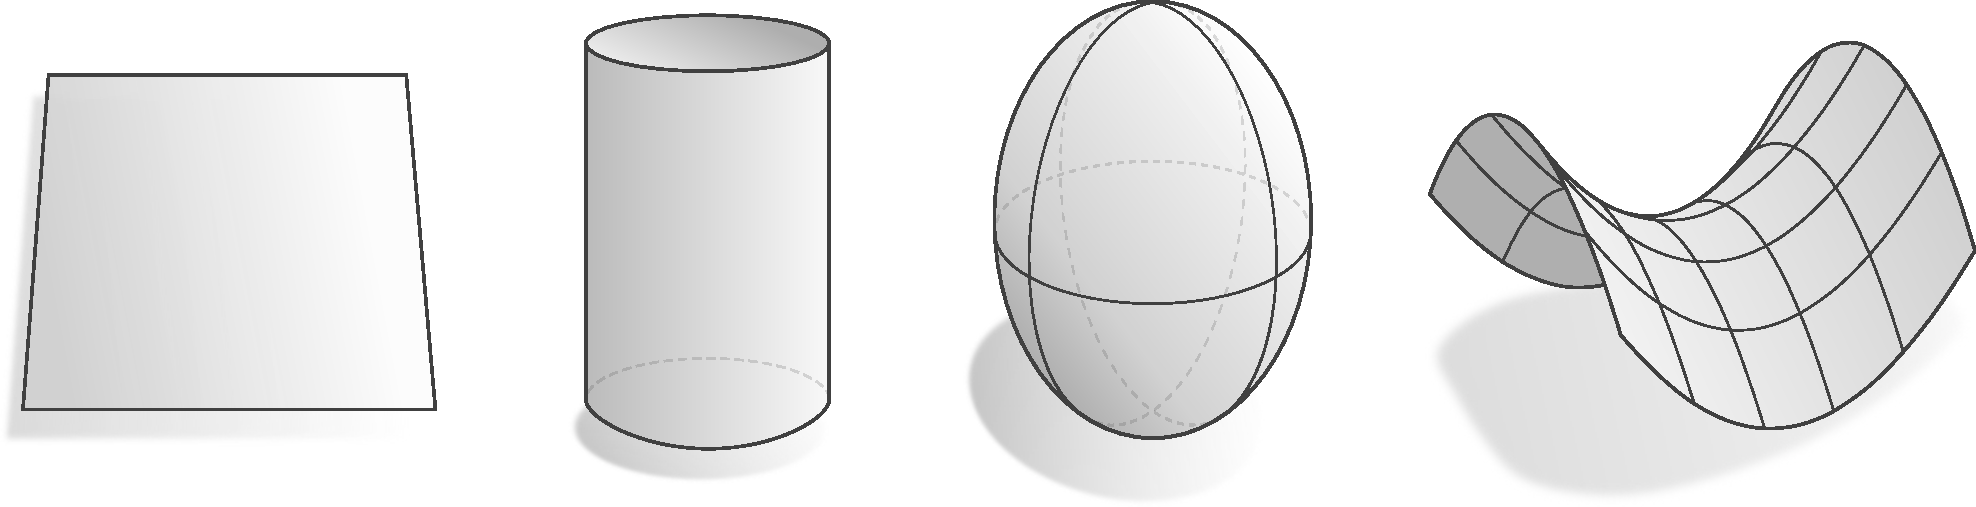
\includegraphics[width=1.\textwidth]{figures/curvature_surfaces.pdf}
    \caption{\small
        سطوح جایگذاری شده با انحناهای خارجی کیفی متفاوت.
        \textit{چپ:}
        صفحه با انحناهای اصلی و گاوسی صفر مشخص می‌شود
        $\kappa_{\max} = \kappa_{\min} = \kappa_{\textup{Gauss}} = 0$.
        \textit{وسط چپ:}
        یک استوانه یک جهت با انحنای مثبت و یک جهت با انحنای صفر دارد، یعنی
        $\kappa_{\max} > 0$ و $\kappa_{\min} = 0$.
        بنابراین انحنای گاوسی آن $\kappa_{\textup{Gauss}} = 0$ نیز صفر است.
        صفحه و استوانه به صورت محلی ایزومتریک هستند، یعنی هندسه ذاتی آنها به صورت محلی قابل تشخیص نیست.
        توجه داشته باشید که صفحه را می‌توان لوله کرد (گسترش داد) تا یک استوانه تشکیل شود -- تفاوت بین این دو فقط در جایگذاری در فضای محیطی است.
        \textit{وسط راست:}
        یک بیضی‌گون با انحناهای اصلی و گاوسی مثبت $\kappa_{\max} > 0$, $\kappa_{\min} > 0$ و $\kappa_{\textup{Gauss}} > 0$ در هر نقطه مشخص می‌شود.
        \textit{راست:}
        سطح یک زین در جهات مخالف خم می‌شود، که دلالت بر علامت‌های مخالف انحناهای اصلی $\kappa_{\max} > 0$ و $\kappa_{\min} < 0$ دارد.
        در نتیجه، انحنای گاوسی $\kappa_{\textup{Gauss}} < 0$ منفی است.
    }
    \label{fig:curvature_surfaces}
\end{figure}

از آنجا که کانولوشن‌های $\GM$ فقط به هندسه ذاتی یک سطح بستگی دارند، خواننده ممکن است تعجب کند که چرا ما در مورد ویژگی‌های خارجی آنها مانند انحناهای اصلی بحث می‌کنیم.
دلیل این است که کانولوشن‌های $\GM$ با این وجود می‌توانند از هندسه خارجی یک سطح مطلع شوند، به عنوان مثال با کدگذاری آن در میدان‌های ویژگی.
هندسه خارجی علاوه بر این ممکن است برای تراز کردن ابتکاری چارچوب‌های یک $\{e\}$-ساختار و در نتیجه کرنل‌ها استفاده شود.
برای مثال، \citet{jin2018learning} و \citet{li2019crossAtlas} چارچوب‌ها را در امتداد محور $z$ فضای محیطی $\R^3$ تراز می‌کنند، در حالی که \citet{boscaini2016learning} و \citet{tatarchenko2018tangent} چارچوب‌ها را در امتداد جهت انحنای اصلی غالب سطح تراز می‌کنند.
توجه داشته باشید که این روش‌های ابتکاری همیشه خوش‌تعریف نیستند:
به عنوان مثال، تصویر محور $z$ روی یک فضای مماس «افقی» (در فضای محیطی) صفر است،
و جهت انحنای اصلی غالب ممکن است تعریف نشده باشد، همانطور که در مورد کره صادق است.






















\subsubsection{هندسه‌ی گسسته‌سازی شده‌ی مش‌های سطحی}
\label{sec:surfaces_geom_mesh}

در اصل، امکان توصیف کانولوشن‌های $\GM$ روی پارامتری‌سازی‌های محلی سطح همانطور که در بخش قبل توصیف شد، وجود دارد.
در حالی که این رویکرد ممکن است برای برخی هندسه‌های ساده یا متقارن مانند بیضی‌گون‌ها، هذلولی‌گون‌ها یا چنبره‌ها مناسب باشد، برای هندسه‌های پیچیده‌تر غیرعملی به نظر می‌رسد.
در عمل، سطوح عمدتاً به صورت گسسته‌سازی شده ارائه می‌شوند، به عنوان مثال به شکل مش‌های مثلثی، مش‌های چهارضلعی، مش‌های نیم-یال، سطوح تقسیمی یا ابرهای نقطه.
به دلیل استفاده گسترده از آنها -- هم به طور کلی و هم به طور خاص در توصیف کانولوشن‌های $\GM$ سطحی که در دو بخش بعدی مرور می‌کنیم -- ما در ادامه عمدتاً بر روی مش‌های مثلثی تمرکز خواهیم کرد.
بنابراین هدف ما برای باقیمانده بخش فعلی این است که کمیت‌ها و تعاریف را از نظریه هموار گرفته و همتایان گسسته آنها را روی مش‌های مثلثی مورد بحث قرار دهیم.
متأسفانه، این آنالوگ‌های گسسته معمولاً یکتا نیستند، به طوری که تعداد زیادی از تعاریف غیرمعادل وجود دارد.%
\footnote{
    \citet{meyer2003discrete} این وضعیت را به این صورت توصیف می‌کند:
    \emph{«علی‌رغم استفاده گسترده از مش‌های مثلثی در گرافیک کامپیوتری، هیچ اتفاق نظری در مورد مناسب‌ترین روش برای تخمین ویژگی‌های هندسی ساده مانند بردارهای نرمال و انحنا روی سطوح گسسته وجود ندارد.»}
    به طور مشابه، \citet{craneDiscreteDifferentialGeometry2014} ادعا می‌کند:
    \emph{«هیچ راه "درست" واحدی برای گسسته‌سازی یک کمیت هندسی داده شده وجود ندارد، بلکه راه‌های مختلف زیادی وجود دارد که هر کدام برای یک هدف خاص مناسب است.»}
}
ما در ادامه سعی خواهیم کرد یک ایده کلی در مورد برخی از رایج‌ترین رویکردها برای گسسته‌سازی هندسه هموار سطوح بر حسب مش‌های مثلثی ارائه دهیم.


\paragraph{توپولوژی، هندسه و جایگذاری مش‌های مثلثی:}
مش‌های مثلثی $(\mathcal{V},\mathcal{F})$ معمولاً بر حسب یک مجموعه از
\begin{align}
    \mathcal{V}\subseteq\N
\end{align}
\emph{رئوس} و یک مجموعه از
\begin{align}
    {\mathcal{F} \subseteq \big\{\mkern-2mu \{i,j,k\} \mkern2mu\big|\mkern2mu i\neq j\neq k \in\mathcal{V} \big\}}
\end{align}
\emph{وجوه} مثلثی کدگذاری می‌شوند،
که این شرط را برآورده می‌کنند که هر رأس حداقل در یکی از وجوه موجود باشد.%
\footnote{
    وجوه به طور جایگزین می‌توانند به عنوان سه‌تایی‌های مرتب از رئوس تعریف شوند.
    ترتیب رئوس (یا بهتر بگوییم، کلاس‌های هم‌ارزی ترتیب‌ها تحت یک تعداد زوج از جایگشت‌ها) ممکن است برای کدگذاری جهت‌گیری وجوه استفاده شود.
    ما در عوض جهت‌گیری وجوه را همانند نظریه هموار خود با انتخاب یک دست‌سانی از چارچوب‌های مرجع کدگذاری خواهیم کرد.
}
یک مجموعه از
\begin{align}
    \mathcal{E} = \big\{ \{i,j\} \,\big|\ i\neq j\in \{i',j',k'\} \textup{ for some } \{i',j',k'\} \in \mathcal{F} \big\}
\end{align}
\emph{یال‌ها} که وجوه را محدود می‌کنند، بلافاصله نتیجه می‌شود.
در عمل، اغلب یک مجموعه از
\begin{align}
    P = \big\{ p_i \in \R^3 \,\big|\, i\in\mathcal{V} \big\}
\end{align}
موقعیت‌های رأس داده می‌شود، که یک \emph{جایگذاری} از مش را در فضای محیطی~$\R^3$ مشخص می‌کند.
این جایگذاری طول‌های
\begin{align}
    l_{\{i,j\}} = \lVert p_j-p_i \rVert
\end{align}
یال‌های $\{i,j\}$ و مساحت‌های
\begin{align}
    \textup{A}_{\{i,j,k\}} = \frac{1}{2} \big\lVert {(p_j-p_i)} \times (p_k-p_i) \big\rVert
\end{align}
وجوه $\{i,j,k\}$ را نتیجه می‌دهد.


ما به طور خاص به \emph{مش‌های سطحی} علاقه‌مندیم، که باید شرایط اضافی را برآورده کنند.
برای فرمول‌بندی این شرایط، توجه داشته باشید که عناصر مش $\{ i_0, \dots, i_n \}$
(که در آن $n=0,1\ \text{or}\ 2$ برای رئوس، یال‌ها یا وجوه است)
$n$-\emph{سادک‌ها} را القا می‌کنند، که به عنوان پوشش‌های محدب
\begin{align}
    \operatorname{convex} \!\big(\{ i_0, \dots, i_n \}\big)\ :=\ 
    \Big\{ \sum\nolimits_{j=0}^n \alpha_j\mkern2mu p_{i_j} \,\Big|\, 
    \sum\nolimits_{j=0}^n \alpha_j = 1\,\ \textup{and}\,\ \alpha_j\geq0\,\ \forall\,j=0,\dots,n \Big\}
    \ \ \subset\ \R^3 \,.
\end{align}
تعریف می‌شوند. مجموعه‌ای که تمام این سادک‌ها (عناصر مش) را در بر می‌گیرد، یک \emph{کمپلکس سادکی-۲ خالص} را تشکیل می‌دهد~\cite{desbrun2005DiscreteExteriorCalculus,craneDiscreteDifferentialGeometry2014}.
اینکه کمپلکس سادکی-۲ \emph{خالص} است به این معنی است که هر سادک-۰ (رأس) و سادک-۱ (یال) زیرمجموعه‌ای از حداقل یک سادک-۲ (وجه) است.
به عبارت دیگر، هیچ رأس یا یال منقطعی در مش وجود ندارد.
\emph{فضای زیربنایی}
\begin{align}
    \bigcup_{\{ i_0, \dots, i_n \} \in \mathcal{V} \cup \mathcal{E} \cup \mathcal{F}}
    \mkern-40mu
    \operatorname{convex} \!\big( \{ i_0, \dots, i_n \}\big)
    \ \ \overset{\textup{(pure)}}{=}\,
    \bigcup_{\{i,j,k\} \in \mathcal{F}}
    \mkern-10mu
    \operatorname{convex} \!\big( \{i,j,k\}\big)
    \ \ \ \subset\ \R^3
\end{align}
از کمپلکس سادکی به عنوان اجتماع تمام سادک‌های آن تعریف می‌شود، که با توپولوژی معمول به عنوان یک زیرمجموعه از~$\R^3$ مجهز شده است.
یک مش سپس یک مش سطحی (مش منیفلد) نامیده می‌شود اگر فضای زیربنایی یک سطح توپولوژیکی (منیفلد)، به صورت اختیاری با مرز، باشد.
به طور شهودی، این امر نیازمند
۱) این است که هر یال مجاور دو وجه (یا یکی در مرزها) باشد و
۲) اینکه وجوه اطراف هر رأس یک دیسک توپولوژیکی (یا یک نیم‌دیسک در مرزها) تشکیل دهند.


چنین مش‌های سطحی تعریف شده، همتایان گسسته سطوح ریمانی \emph{جایگذاری شده} هستند.
با این حال، از آنجا که کانولوشن‌های $\GM$ مستقل از هندسه \emph{خارجی} منیفلد زیربنایی هستند، بحث مختصر در مورد هندسه \emph{ذاتی} آنها آموزنده است.
بنابراین مجموعه‌های رأس، یال و وجه $\mathcal{V}$، $\mathcal{E}$ و $\mathcal{F}$ را در نظر بگیرید، اما مکان‌های جایگذاری $P$ رئوس را کنار بگذارید.
در مجموع، این مجموعه‌ها یک \emph{کمپلکس سادکی-۲ انتزاعی}
$\mathcal{V} \cup \mathcal{E} \cup \mathcal{F} \,,$
را تشکیل می‌دهند که به عنوان خانواده‌ای از سادک‌های انتزاعی $\{i_0,\dots,i_n\}$ که تحت عمل زیرمجموعه‌گیری بسته است، تعریف می‌شود~\cite{craneDiscreteDifferentialGeometry2014}.
اگر این کمپلکس سادکی-۲ (که اکنون انتزاعی است)
۱) خالص و
۲) به گونه‌ای باشد که «ستاره» هر رأس (که با سادک‌های حاوی آن رأس داده می‌شود) یک دیسک ترکیبیاتی تشکیل دهد،
این یک \emph{سطح سادکی انتزاعی} را تشکیل می‌دهد (که دقیقاً در صورتی است که مش جایگذاری شده یک مش سطحی باشد).
سطوح سادکی انتزاعی را می‌توان به عنوان همتایان ترکیبیاتی منیفلدهای توپولوژیکی در نظر گرفت.
آنها امکان محاسبه ناورداهای توپولوژیکی، به عنوان مثال مشخصه اویلر
\begin{align}
    \mathcal{X}_{\textup{Euler}} = |\mathcal{V}|-|\mathcal{E}|+|\mathcal{F}| \,.
\end{align}
را می‌دهند. به عنوان یک ناوردای توپولوژیکی، مشخصه اویلر برای هر دو فضای همسان‌ریخت، به ویژه برای یک منیفلد هموار و هر یک از مثلث‌بندی‌های آن، برابر است.
برای مثال، بیست‌وجهی از بخش~\ref{sec:spherical_CNNs_icosahedral} دارای $\mathcal{X}_{\textup{Euler}}^\textup{ico} = 12-30+20 = 2$ است، که با $\mathcal{X}_{\textup{Euler}}^{S^2} = 2$ برای کره ۲-بعدی مطابقت دارد.


برای رسیدن به یک توصیف ذاتی از \emph{هندسه} یک سطح مثلث‌بندی شده، به یال‌های $\{i,j\} \in \mathcal{E}$ \emph{طول یال} ${l_{ij} \in \R^+}$ اختصاص می‌دهیم.
برای سازگاری، این طول‌ها باید نامساوی مثلث $l_{\{i,j\}} + l_{\{j,k\}} > l_{\{k,i\}}$ را برای هر وجه $\{i,j,k\} \in \mathcal{F}$ برآورده کنند.
طول یال‌ها متریک‌های اقلیدسی (توابع فاصله) را روی وجوه و بنابراین یک متریک اقلیدسی تکه‌ای-تعریف شده را روی کل سطح القا می‌کنند.
این متناظر با یک متریک ریمانی (یا فرم بنیادی اول) است که دور از رئوس اقلیدسی و در یک همسایگی کوچک حول رئوس «مخروط‌مانند» (تکین) است~\cite{Crane2020DiscreteConformalGeometry,desbrun2005DiscreteExteriorCalculus}.


برای بستن دایره به تعریف خارجی اولیه ما از مش‌های مثلثی، باید مش را در فضای محیطی~$\R^3$ جایگذاری کرد.
اطلاعات لازم در مورد هندسه خارجی با مجهز کردن مش به یک \emph{فرم بنیادی دوم} داده می‌شود.
در محیط گسسته، این فرم را می‌توان به عنوان یک انتخاب از زاویه دووجهی (زاویه خمش) بین هر دو مثلث مجاور، یعنی یک زاویه برای هر یال غیرمرزی مش، تعریف کرد.
با فرض اینکه این داده‌ها به طور سازگار انتخاب شده باشند%
\footnote{
    فرم‌های بنیادی اول و دوم گسسته باید یک شرط انتگرال‌پذیری را برآورده کنند،
    مشابه معادله گاوس و معادلات مایناردی-کوداتسی در محیط هموار~\cite{wang2012surfaceReconstruction}.
},
امکان بازسازی جایگذاری، یعنی موقعیت‌های رأس~$P$, تا حرکات صلب در~$\E3$ وجود دارد~\cite{lipman2005linear,wang2012surfaceReconstruction}.
در حالی که یک جایگذاری از سطح برای کانولوشن‌های $\GM$ ذاتی ضروری نیست، تمام مقالات فهرست شده در ردیف‌های (۳۷-۴۱) جدول~\ref{tab:network_instantiations} مدل‌های خود را روی مش‌های مثلثی جایگذاری شده ارزیابی می‌کنند.



\paragraph{فضاهای مماس و میدان‌های برداری:}
برای توصیف میدان‌های برداری روی مش‌ها، و برای مجهز کردن مش‌ها به ساختار هندسی مانند اتصالات، لازم است یک مفهوم از فضاهای مماس که به آنها متصل هستند، تعریف شود.
تعاریف ناسازگار متعددی، که برای کاربرد خاص مورد نظر طراحی شده‌اند، در مقالات وجود دارد.
از آنجا که میدان‌های برداری معمولاً در مکان‌های گسسته نمونه‌برداری می‌شوند، کلاف‌های مماس گسسته اغلب فقط به صورت جزئی تعریف می‌شوند، به عنوان مثال فقط روی وجوه، یال‌ها یا رئوس.
ما به طور خلاصه برخی از این تعاریف را مرور می‌کنیم، یک بررسی دقیق‌تر را می‌توان در~\cite{deGoes2016VectorFieldProcessing} یافت.


از آنجا که وجوه (سادک‌های-۲) یک مش جایگذاری شده تخت هستند، می‌توان به طور طبیعی فضاهای مماس آنها را به عنوان آن دسته از زیرفضاهای دوبعدی~$\R^3$ که در آنها قرار دارند، تعریف کرد~\cite{craneTrivialConnectionsDiscrete2010,craneDiscreteDifferentialGeometry2014,wang2012surfaceReconstruction}.
به طور خاص، با توجه به یک وجه $\{i,j,k\} \in \mathcal{F}$، می‌توان فضاهای مماس $\TpM = \operatorname{span}(p_j-p_i,\, p_k-p_i) \subset \R^3$ را برای هر $p\in \operatorname{convex}\!\big(\{i,j,k\}\big)$ به عنوان \emph{پوشش خطی هر دو بردار یال} تعریف کرد.
تراز فضای مماس در فضای محیطی اغلب بر حسب نرمال وجه $n = (p_j-p_i) \times (p_k-p_i)$ نمایش داده می‌شود.
میدان‌های برداری مماس (یا ویژگی) گسسته در نمایش‌های مبتنی بر وجه را می‌توان به عنوان ثابت روی هر وجه تعریف کرد، یعنی با یک بردار مماس (یا ویژگی) منفرد برای هر وجه نمایش داده می‌شوند.
نسبت به یک انتخاب از چارچوب مرجع روی هر یک از وجوه، چنین میدان‌های برداری مماس و ویژگی به ترتیب با $2|\mathcal{F}|$ یا $c|\mathcal{F}|$ ضریب برداری کدگذاری می‌شوند.
توجه داشته باشید که چنین میدان‌های برداری به رئوس یا یال‌ها گسترش نمی‌یابند.
به دلیل ناپیوستگی آنها، مفهوم عملگرهای دیفرانسیل، که بر روی چنین میدان‌هایی عمل می‌کنند، بسیار محدود است~\cite{deGoes2016VectorFieldProcessing} (که برای کاربرد خاص ما بی‌اهمیت است).
یک طرح درون‌یابی خطی از میدان‌های برداری مبتنی بر وجه در~\cite{li2006representing} پیشنهاد شده است.


از آنجا که هیچ جهت نرمال طبیعی در رئوس یک مش وجود ندارد، تعاریف رایج متعددی برای فضاهای مماس رأس وجود دارد.
\emph{نرمال‌های رأس} را می‌توان به عنوان مثال به عنوان میانگین وزن‌دار مساحتی از نرمال‌های وجوه مجاور تعریف کرد~\cite{lipman2005linear,lai2009metric,deHaan2020meshCNNs}.
علاوه بر وزن‌دهی مساحتی، گاهی از وزن‌های یکنواخت یا وزن‌های زاویه نوک استفاده می‌شود~\cite{craneDiscreteDifferentialGeometry2014}.
گزینه دیگر، تعریف بردارهای نرمال از طریق یک عملگر نرمال انحنای میانگین است \cite{meyer2003discrete}.
نرمال حاصل با نرمال‌های مشتق شده از طریق گرادیان‌های مساحت مطابقت دارد، اما با آنهایی که از طریق گرادیان‌های حجم یا نرمال‌های کره محاطی مشتق شده‌اند، متفاوت است؛ به~\cite{craneDiscreteDifferentialGeometry2014} مراجعه کنید.


به طور جایگزین، می‌توان فضاهای مماس رأس را به روش \emph{ذاتی} تعریف کرد، به سادگی با تعریف آنها به عنوان فضاهای برداری دوبعدی که به رأس متصل هستند.
رابطه آنها با هندسه مش در یک همسایگی محلی حول رأس در اینجا با نمایش همسایگی یک-حلقه در صفحات مماس کدگذاری می‌شود.
مسلماً برجسته‌ترین این رویکردها بر اساس تغییر مقیاس زاویه کل
\begin{align}\label{eq:mesh_total_incident_angle}
    \Theta_i \,=\! \sum_{\{i,j,k\}\in\mathcal{F}} \theta_{\{i,j,k\}}^i \,,
\end{align}
است، که از زوایای نوک
$\theta_{\{i,j,k\}}^i = \arccos \big\langle \frac{p_j-p_i}{\lVert p_j-p_i\rVert} \frac{p_k-p_i}{\lVert p_k-p_i\rVert} \big\rangle$
از تمام مثلث‌های $\{i,j,k\}$ مجاور رأس $i\in\mathcal{V}$ جمع می‌شود.
اگر این زاویه دقیقاً $2\pi$ باشد، همسایگی محلی حول رأس به طور ذاتی تخت است؛ به عنوان مثال به همسایگی قرمز یا سبز در شکل~\ref{fig:ico_neighborhoods} مراجعه کنید.
یک زاویه $\Theta_i < 2\pi$ همانند همسایگی آبی، نشان‌دهنده یک انحنای گاوسی گسسته مثبت (که به درستی در ادامه تعریف می‌شود) $\kappa_{\textup{Gauss},i} = 2\pi - \Theta_i$ است، یعنی یک همسایگی مخروط‌مانند.
یک زاویه $\Theta_i > 2\pi$ به طور مشابه متناظر با یک همسایگی زین‌مانند با انحنای گاوسی منفی است.
رویکرد دنبال شده در
\cite{polthier1998straightest,zhang2006vectorFieldDesign,Knoppel:2013:GOD,Sharp2019VectorHeatMethod,craneDiscreteDifferentialGeometry2014}
این است که همسایگی یک-حلقه را با تغییر مقیاس همسانگرد \emph{زوایای قطبی} با ضریب $s_i = \frac{2\pi}{\Theta_i}$ به کل $s_i \Theta_i = 2\pi$ از یک فضای اقلیدسی (مماس) \emph{پهن} کنند.
یک میدان برداری در این محیط با یک بردار برای هر رأس نمایش داده می‌شود.
یک انتخاب از پیمانه، که اغلب با یکی از یال‌ها تراز شده است، سپس امکان کدگذاری میدان‌های برداری مماس یا ویژگی را به ترتیب بر حسب $2|\mathcal{V}|$ یا $c|\mathcal{V}|$ ضریب فراهم می‌کند.
\citet{zhang2006vectorFieldDesign} پیشنهاد کردند که بردارها را با یک تابع وزن‌دهی کلاهی تکه‌ای-خطی از رئوس به وجوه درون‌یابی کنند.
جهت بردارها در اینجا با یک انتقال اقلیدسی معمول روی فضاهای مماس پهن شده تعیین می‌شود.
همانطور که توسط~\citet{deGoes2016VectorFieldProcessing} اشاره شده است، این درون‌یابی پیوسته نیست.
برای حل این مشکل، همان نویسندگان در \cite{liu2016discreteConnection} پیشنهاد می‌کنند که یک ساختار هموار را روی مش مثلثی تعریف کرده و همسایگی‌های یک-حلقه را در \emph{چارت‌های هموار} نمایش دهند.
سپس یک درون‌یابی هموار با انتقال بردارها از طریق یک اتصال سادکی هموار روی مش انجام می‌شود، که برای نزدیکترین حالت ممکن به اتصال لوی-چیویتا القا شده از فضای جایگذاری اصلی، بهینه‌سازی شده است.
توجه داشته باشید که هر دو رویکرد به طور موثر هندسه را حول رئوس پهن می‌کنند، یعنی دقیقاً روی مش مثلثی عمل نمی‌کنند.


یک رویکرد دیگر، که ریشه در حساب دیفرانسیل خارجی گسسته دارد~\cite{desbrun2005DiscreteExteriorCalculus,elcott2005building}، تعریف بردارهای مماس $v = \omega^\sharp \in \TpM$ بر حسب \emph{۱-فرم‌ها} $\omega \in \TspM$ با استفاده از ایزومورفیسم موسیقیایی (وابسته به متریک) $\sharp^\eta: \TsM \to \TM$ («بالا بردن اندیس») است.
از آنجا که ۱-فرم‌های سادکی به طور طبیعی به \emph{یال‌ها} (سادک‌های-۱) اختصاص داده می‌شوند، این منجر به میدان‌های برداری می‌شود که بر حسب یک بردار برای هر یال و در نتیجه $2|\mathcal{E}|$ ضریب پس از انتخاب چارچوب‌ها، پارامتری می‌شوند.
با این حال، همانطور که توسط \citet{deGoes2016VectorFieldProcessing} استدلال شده است، یک درون‌یابی تکه‌ای-خطی از بردارها روی وجوه دوباره به ناپیوستگی منجر خواهد شد.
علاوه بر این، برای ما روشن نیست که چگونه این رویکرد می‌تواند به کلاف‌های برداری همبسته عمومی و در نتیجه میدان‌های ویژگی تعمیم یابد.







با توجه به هر یک از ساختارهای بالا از فضاهای مماس، \emph{چارچوب‌های مرجع محلی} به راحتی به عنوان زوج‌های مرتبی از بردارهای مماس خطی مستقل تعریف می‌شوند.
یک انتخاب رایج در اینجا تراز کردن اولین محور چارچوب با یکی از یال‌های مجاور سادک فعلی (عنصر مش) است.
به طور خاص برای مورد چارچوب‌های راست‌هنجار و راست‌گرد، یعنی هر زمان که $G\leq\SO2$ باشد، یک انتخاب از یال (جهت‌دار) یک چارچوب را به طور کامل تعیین می‌کند.
سپس بردارهای مماس اغلب در مختصات قطبی نمایش داده می‌شوند، با زاویه اندازه‌گیری شده نسبت به یال مرجع.
اگر فضاهای مماس به صورت خارجی مدل‌سازی شوند، یعنی به عنوان زیرفضاهای دوبعدی از فضای محیطی $\R^3$، رایج‌ترین روش نمایش صریح چارچوب‌ها به عنوان یک زوج مرتب از بردارها در $\TpM \subset \R^3$ است.
تعاریف چارچوب‌ها و پیمانه‌ها سپس کاملاً معادل تعاریف در
معادلات~\eqref{eq:embedding_gauge_map_orthonormal_frame} و~\eqref{eq:embedding_space_R3_frame}
در بخش~\ref{sec:sphere_geometry} هستند.

$G$-ساختارها، طبق معمول، به عنوان کلاف‌هایی از چارچوب‌ها تعریف می‌شوند، که در هر فضای مماس از طریق تبدیلات پیمانه‌ای با مقادیر $G$ به هم مرتبط هستند.
در جامعه گرافیک کامپیوتری، علاقه خاصی به \emph{$N$-میدان‌های جهتی} (یا میدان‌های $N$-RoSy واحد) وجود دارد، که در آنجا به عنوان مجموعه‌ای از $N$ میدان برداری واحد تعریف می‌شوند، به طوری که $N$ بردار در هر فضای مماس با زاویه $2\pi/N$ از هم فاصله دارند.
از آنجا که هر بردار واحد روی یک منیفلد جهت‌پذیر یک چارچوب راست‌هنجار و راست‌گرد متناظر را القا می‌کند، دیده می‌شود که $N$-میدان‌های جهتی معادل $\operatorname{C}_N$-ساختارها هستند.
یک مثال، $\operatorname{C}_6$-ساختار روی بیست‌وجهی در شکل~\ref{fig:G_structure_ico_3} است، که به طور موثر $6$ جهت واحد را به هر نقطه اختصاص می‌دهد، به جز در قطب‌ها، که در آنجا تکینگی‌هایی با اندیس $\frac{1}{6}$ (یا زاویه $\frac{2\pi}{6}$) دارد.
طراحی تعاملی میدان‌های جهتی هموار، با تکینگی‌های تعریف شده توسط کاربر در میان دیگر محدودیت‌ها، یک زمینه تحقیقاتی فعال در جامعه گرافیک کامپیوتری است
\cite{li2006representing,ray2008nSymmDirectionField,lai2009metric,craneTrivialConnectionsDiscrete2010,Knoppel:2013:GOD,liu2016discreteConnection,Sharp2019VectorHeatMethod}.
برخی از کانولوشن‌های $\GM$ سطحی که در بخش بعدی مرور می‌کنیم از چنین الگوریتم‌هایی برای محاسبه یک $\operatorname{C}_N$-ساختار استفاده می‌کنند~\cite{huang2019texturenet,Yang2020parallelFrameCNN}.



\paragraph{متریک ریمانی و ایزومتری‌ها:}
با داشتن یک مش مجهز به فضاهای مماس، می‌توان یک \emph{متریک ریمانی} را روی آن تعریف کرد.
رایج‌ترین مورد، مش‌های جایگذاری شده ایزومتریک با فضاهای مماس مدل‌سازی شده به عنوان زیرفضاهای دوبعدی از فضای محیطی~$\R^3$ است.
همانطور که قبلاً در معادلات~\eqref{eq:spherical_embedding_metric_explicit} و~\eqref{eq:surface_embedding_metric} توصیف شد، متریک سپس با تحدید حاصلضرب داخلی استاندارد اقلیدسی $\langle\cdot,\cdot\rangle_{\R^3}$ از فضای جایگذاری به فضاهای مماس القا می‌شود.

اگر فضاهای مماس به صورت ذاتی مدل‌سازی شوند، یک متریک را می‌توان با انتخاب یک $\O{d}$-ساختار، یعنی چارچوب‌های مرجعی که \emph{تعریف} شده‌اند راست‌هنجار باشند، ثابت کرد.
کمی کمتر از همان‌گویی، اگر طول یال‌ها~$l_{\{i,j\}}$ و بنابراین یک تابع فاصله اقلیدسی تکه‌ای-تعریف شده روی سطح داده شده باشد، انتخاب $\O{d}$-ساختار باید با این طول‌ها سازگار باشد.
به طور خاص، نگاشت لگاریتمی باید منجر به بردارهای مماس با نرم (ریمانی) $|\log_p(q)| = \mathscr{d}$ شود اگر نقاط $p$ و~$q$ با یک فاصله اقلیدسی $\mathscr{d} \in \R^+$ از هم جدا شده باشند.
توجه داشته باشید که این گزاره نیازمند یک تعریف سازگار از اتصال لوی-چیویتا روی مش است، که در ادامه به آن می‌پردازیم.


\emph{ایزومتری‌ها} به طور ذاتی طبق معمول تعریف می‌شوند، یعنی به عنوان آن دسته از نگاشت‌های مش به خود، که متریک را حفظ می‌کنند.
به صورت خارجی، گروه ایزومتری از آن دسته از ایزومتری‌های $\phi \in \E2$ فضای جایگذاری تشکیل شده است که مش را ناوردا باقی می‌گذارند.
اکثر مقالات در
ردیف‌های (۳۷-۴۱)
از جدول~\ref{tab:network_instantiations}
مجموعه داده‌هایی را در نظر می‌گیرند که مش‌های آنها دارای یک گروه ایزومتری بدیهی هستند.
با این حال، همسایگی‌های محلی مش‌ها اغلب با این وجود با یکدیگر ایزومتریک (یا تقریباً ایزومتریک) هستند، که در شکل~\ref{fig:suzanne_local_isometry} مثال زده شده است.
همانطور که در بخش~\ref{sec:isometry_groups} بحث شد، هموردایی ایزومتری کانولوشن‌های $\GM$ همچنان به صورت محلی برقرار خواهد بود اگر میدان دید کرنل‌ها به اندازه کافی کوچک باشد.







\paragraph{اتصالات، انتقال‌دهنده‌ها و ژئودزیک‌ها روی مش‌های مثلثی:}
آخرین جزء مورد نیاز ما برای پیاده‌سازی کانولوشن‌های $\GM$ روی مش‌ها، پول‌بک انتقال‌دهنده $\Expsp$ از میدان‌های ویژگی است (معادله~\eqref{eq:transporter_pullback_in_coords}).
بنابراین ما باید بدانیم که چگونه
۱) بردارهای ویژگی را به صورت موازی روی مش‌ها منتقل کنیم و
۲) ژئودزیک‌ها را روی مش‌ها، به ویژه نگاشت نمایی یا، بسته به پیاده‌سازی، نگاشت لگاریتمی را محاسبه کنیم.
تمام این نگاشت‌ها در نهایت به یک انتخاب از \emph{اتصال} روی مش بستگی دارند.
در محیط هموار، یک اتصال اساساً مجموعه‌ای از انتقال‌دهنده‌های بی‌نهایت کوچک بین فضاهای مماس مجاور است.
بنابراین اتصالات گسسته روی مش‌ها معمولاً به عنوان انتقال‌دهنده‌ها بین عناصر مش مجاور تعریف می‌شوند.
انتخاب خاص گسسته‌سازی کلاف مماس، که گزینه‌های آن در بالا مورد بحث قرار گرفت، بر تعریف خاص اتصال تأثیر می‌گذارد.
در ادامه، ما برخی از گسسته‌سازی‌های اتصالات را که در مقالات یافت می‌شوند، مرور می‌کنیم و توضیح می‌دهیم که چگونه می‌توان از آنها برای محاسبه انتقال‌دهنده‌ها و ژئودزیک‌ها استفاده کرد.


ساده‌ترین مورد برای بررسی، انتقال یا اتصال بین دو وجه مجاور است.
به یاد بیاورید که انتقال لوی-چیویتا روی یک صفحه تخت به عنوان جابجایی یک بردار به گونه‌ای تعریف می‌شود که در معنای معمول اقلیدسی موازی باقی بماند؛ به شکل~\ref{fig:transport_flat} مراجعه کنید.
از آنجا که اتصالات ذاتاً ذاتی هستند، به جایگذاری خاص این صفحه در فضای محیطی بستگی ندارند، که به ما می‌گوید چگونه روی هر سطح گسترش‌پذیر منتقل کنیم.
این به طور خاص به ما می‌گوید که چگونه بین دو مثلث مجاور منتقل کنیم، زیرا می‌توان آنها را باز کرد (گسترش داد) و به یک صفحه تبدیل کرد، همانطور که در شکل~\ref{fig:transport_mesh} به تصویر کشیده شده است.
بنابراین اتصال لوی-چیویتا بین وجوه را می‌توان به این صورت تصور کرد که
۱)~وجوه را پهن کرده،
۲)~بردار را طبق معمول روی صفحه منتقل کرده و
۳)~وجوه را به جایگذاری اصلی خود بازگردانیم~\cite{craneTrivialConnectionsDiscrete2010,mitchell1987discrete,craneDiscreteDifferentialGeometry2014}.
انتقال‌دهنده حاصل
$\mathcal{P}_{\mkern-2mu\overset{}{\protect\scalebox{.62}{$\!T\!M$},\protect\scalebox{.68}{$\{i,j,k\mkern-1mu\}\!\to\!\{i,j,l\}$}}}$
بین وجوه $\{i,j,k\}$ و $\{i,j,l\}$ را می‌توان به صورت اختیاری بر حسب یک عضو گروه
$g^{A\widetilde{A}}_{\protect\scalebox{.68}{$\{i,j,k\mkern-1mu\}\!\to\!\{i,j,l\}$}}$ در~$\GL{2}$ بیان کرد.
از آنجا که اتصال لوی-چیویتا یک اتصال متریک است، برای مورد خاص چارچوب‌های راست‌هنجار منجر به اعضای گروه در~$\O2$ و برای چارچوب‌های راست‌هنجار جهت‌دار منجر به اعضای $\SO2$ یا زوایای دوران می‌شود.

\begin{figure}
    \centering
    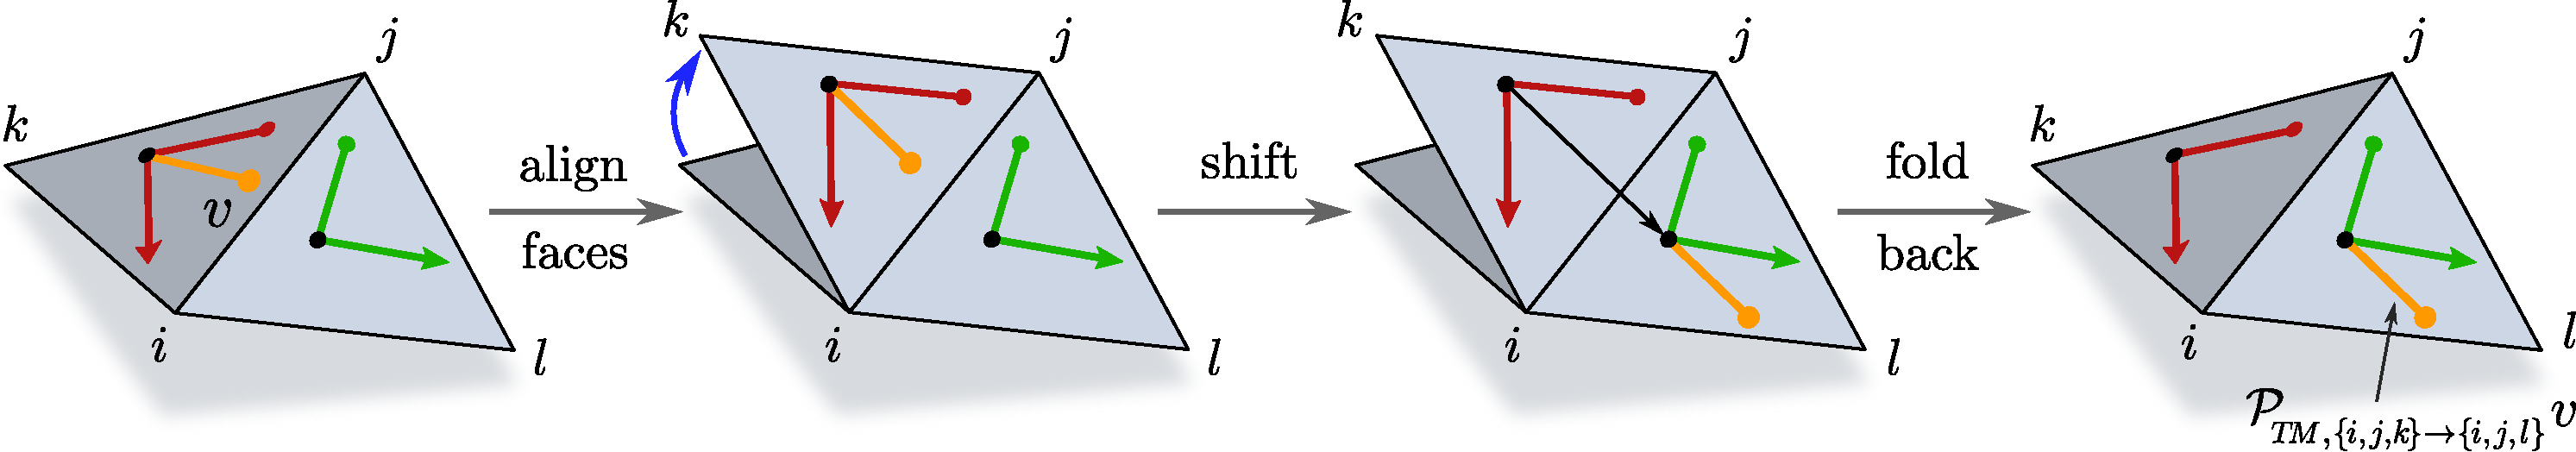
\includegraphics[width=1.\textwidth]{figures/transport_mesh.pdf}
    \caption{\small
        انتقال موازی بین وجوه مش.
        هندسه محلی دو وجه مجاور گسترش‌پذیر است، یعنی به طور ذاتی تخت است و می‌توان آن را به یک صفحه باز کرد.
        بنابراین انتقال لوی-چیویتا بین وجوه با جابجایی یک بردار روی وجوه باز شده و سپس خم کردن وجوه به جایگذاری اصلی خود داده می‌شود.
        این انتقال موازی بین وجوه مجاور را می‌توان به عنوان آنالوگ گسسته اتصال لوی-چیویتا پیوسته در محیط هموار در نظر گرفت~\cite{craneTrivialConnectionsDiscrete2010}.
        با توجه به هر انتخاب از چارچوب‌های مرجع، انتقال
        $\mathcal{P}_{\mkern-2mu\overset{}{\protect\scalebox{.62}{$\!T\!M$},\protect\scalebox{.68}{$\{i,j,k\mkern-1mu\}\!\to\!\{i,j,l\}$}}}$
        با یک عضو گروه
        $g^{A\widetilde{A}}_{\protect\scalebox{.68}{$\{i,j,k\mkern-1mu\}\!\to\!\{i,j,l\}$}} \in \GL{2}$ (یا $\SO2$ هنگام در نظر گرفتن چارچوب‌های راست‌هنجار و راست‌گرد) نمایش داده می‌شود.
        اتصالات عمومی‌تر یک تبدیل خطی اضافی را به بردار مستقل از مختصات هنگام انتقال بین وجوه اعمال می‌کنند.
        تعاریف جایگزین از اتصالات گسسته، به عنوان مثال برای انتقال بین رئوس در امتداد یال‌ها، در متن اصلی مورد بحث قرار گرفته‌اند.
    }
    \label{fig:transport_mesh}
\end{figure}


همانطور که توسط \citet{craneTrivialConnectionsDiscrete2010} پیشنهاد شده است، امکان تعمیم این ساختار فراتر از اتصالات لوی-چیویتا وجود دارد:
به جای صرفاً جابجایی بردارها بین وجوه پهن شده، اتصالات عمومی‌تر یک تبدیل خطی اضافی، به عنوان مثال یک دوران اضافی، را اعمال می‌کنند.
در حالی که این تبدیل اضافی با یک تبدیل متناظر از عبارت مختصاتی انتقال‌دهنده
$g^{A\widetilde{A}}_{\protect\scalebox{.68}{$\{i,j,k\mkern-1mu\}\!\to\!\{i,j,l\}$}}$
منعکس خواهد شد، از نظر مفهومی از آن مستقل است و می‌تواند در یک چارچوب کاملاً مستقل از مختصات تعریف شود.
نویسندگان از این ایده برای ساخت اتصالات بدیهی هموار استفاده می‌کنند، که با داشتن یک انتقال با هولونومی صفر حول هر حلقه ممکن تعریف می‌شوند، و برای هر چه هموارتر بودن بهینه شده‌اند، به جز در برخی تکینگی‌ها که به صورت توپولوژیکی تحمیل شده‌اند~\cite{craneTrivialConnectionsDiscrete2010}.
آنها علاوه بر این اتصالات را در نظر می‌گیرند که دوران‌های (مستقل از مختصات) با $\frac{2\pi}{N}$ را اعمال می‌کنند و می‌توانند برای ساخت $N$-میدان‌های جهتی، متناظر با $\operatorname{C}_N$-ساختارها استفاده شوند.
در کاربردهای ما، ما \emph{همیشه} اتصالات لوی-چیویتا را برای محاسبه ژئودزیک‌ها در نظر خواهیم گرفت.
مدل‌های مرور شده در بخش بعدی~\ref{sec:so2_surface_conv} یک گروه ساختاری $G=\SO2$ را روی مش‌های جهت‌پذیر فرض می‌کنند و از انتقال‌دهنده‌های لوی-چیویتا برای بردارهای ویژگی استفاده می‌کنند.
در مقابل، مدل‌های بخش~\ref{sec:e_surface_conv} یک گروه ساختاری بدیهی $G=\{e\}$ را فرض می‌کنند و بنابراین فقط به اتصالات بدیهی $\{e\}$-ساختار سازگار اجازه می‌دهند.
آنها ویژگی‌ها را به گونه‌ای منتقل می‌کنند که بردارهای ضریب آنها نسبت به چارچوب‌های $\{e\}$-ساختار ناوردا باقی بمانند، یعنی صرفاً مقادیر عددی آنها را کپی می‌کنند.


با توجه به فضاهای مماس جایگذاری شده $\TpM \subset \R^3$ در دیگر عناصر مش مانند رئوس یا یال‌ها، این رویکرد به طور طبیعی به انتقال بین عناصر مش دلخواه تعمیم می‌یابد~\cite{deHaan2020meshCNNs}:
به جای تراز کردن وجوه، می‌توان به عنوان مثال فضای مماس رأس را با وجه مجاور قبل از جابجایی بردار تراز کرد.
از نظر هندسی، این عملیات را می‌توان به عنوان انتقال روی یک مش که رئوس و یال‌های آن در یک همسایگی بی‌نهایت کوچک بریده شده و با یک وجه چندضلعی جایگزین شده‌اند، در نظر گرفت.


یک تعریف جایگزین از اتصالات گسسته در \cite{Knoppel:2013:GOD} و \cite{Sharp2019VectorHeatMethod} ارائه شده است.
نویسندگان هر دو مقاله، فضاهای مماس را فقط در رئوس مدل می‌کنند، جایی که آنها بر حسب تغییر مقیاس زاویه کل ورودی، معادله~\eqref{eq:mesh_total_incident_angle}، به $2\pi$ تعریف می‌شوند، همانطور که در بالا بحث شد.
یک اتصال روی مش سپس با انتقال‌دهنده‌ها روی تمام یال‌های $\{i,j\} \in\mathcal{E}$ داده می‌شود، که فضاهای مماس رئوس مجاور را به هم متصل می‌کنند.
از آنجا که مفهوم هندسی باز کردن مثلث‌ها در اینجا وجود ندارد، انتقال‌دهنده‌های یال از طریق اعضای گروه نسبت به یک چارچوب مبدأ و مرجع کدگذاری می‌شوند.
به طور خاص برای اتصال لوی-چیویتا، و چارچوب‌های مرجع راست‌هنجار و راست‌گرد، این اعضای گروه در~$\SO2$ قرار دارند.
سودمندی این ساختار برای انتقال مستقیم در امتداد مسیرهای دلخواه روی منیفلد نامشخص است، با این حال، برای حل معادلات دیفرانسیل جزئی که به مشتق هموردا بستگی دارند، مفید است.
\citet{Sharp2019VectorHeatMethod} نشان دادند که یک راه‌حل از معادله گرمای برداری با این وجود اجازه می‌دهد تا از چنین اتصالات برای محاسبه (غیرمستقیم) انتقال موازی بین نقاط دلخواه روی یک مش استفاده شود.
\citet{liu2016discreteConnection} یک ساختار دیگر، یعنی اتصالات سادکی هموار بین و در داخل تمام عناصر مش را پیشنهاد می‌کنند.
آنها علاوه بر این بحث می‌کنند که چگونه چنین اتصالات را می‌توان بهینه کرد تا حد ممکن به اتصال لوی-چیویتا (ناهموار) نزدیک باشند.


یک اتصال داده شده، \emph{انتقال موازی} را در امتداد یک مسیر تعیین می‌کند.
در محیط هموار، که اتصالات انتقال‌دهنده‌های بی‌نهایت کوچک هستند، انتقال متناهی با انتگرال‌گیری از اتصال در امتداد مسیر محاسبه می‌شود.
در محیط گسسته، انتقال بر این اساس با ترکیب تبدیلات منفردی که اتصال را بین عناصر مش که توسط مسیر عبور می‌کنند، تشکیل می‌دهند، داده می‌شود.
برای اتصال لوی-چیویتا، این فرآیند متناظر با پهن کردن تمام عناصر مش در امتداد مسیر و سپس جابجایی بردار روی آن است؛ به شکل ۷ در~\cite{lai2009metric} مراجعه کنید.
روش مبتنی بر معادله گرمای برداری توسط \citet{Sharp2019VectorHeatMethod} انتقال بردارها را به طور خاص در امتداد ژئودزیک‌ها محاسبه می‌کند.
از آنجا که این روش برای انتقال از یک مکان مبدأ به \emph{هر} مکان دیگر روی منیفلد به طور همزمان حل می‌کند، این رویکرد می‌تواند کارآمدتر از انتگرال‌گیری از انتقال برای هر مسیر منفرد به طور جداگانه باشد.


\emph{انحنای یک اتصال} در محیط هموار به عنوان هولونومی انتقال آن حول یک دیسک بی‌نهایت کوچک تعریف می‌شود.
انحنا در یک رأس در محیط گسسته به طور مشابه به عنوان هولونومی انتقال حول این رأس تعریف می‌شود.
برای اتصال لوی-چیویتا، این فقط انحنای گاوسی است، که با نقص زاویه
\begin{align}
    \kappa_{\textup{Gauss},i} \,=\, \delta_i \,=\, 2\pi - \Theta_i \,,
\end{align}
داده می‌شود، که در آن $\Theta_i$ زاویه کل نوک از معادله~\eqref{eq:mesh_total_incident_angle} است.
ما دوباره به بیست‌وجهی به عنوان مثال اشاره می‌کنیم، که در همه جا انحنای صفر دارد، به جز در دوازده رأس اصلی خود، که در آن نقص زاویه (انحنا) برابر با~$\frac{2\pi}{6}$ است.
اتصالات بدیهی بنا به ساختار، انحنای صفر دارند.


در آخر، ما باید \emph{ژئودزیک‌ها} را مورد بحث قرار دهیم.
در محیط هموار، ژئودزیک‌ها به عنوان \emph{مستقیم‌ترین مسیرها} تعریف می‌شوند، که با این گزاره رسمیت می‌یابد که مشتقات هموردای بردارهای مماس آنها در امتداد منحنی صفر می‌شوند، یعنی $\nabla_{\dot{\gamma}} \dot{\gamma} = 0$.
این معادل این الزام است که انتقال یک بردار مماس $\dot{\gamma}(t_0)$ در امتداد ژئودزیک، مماس بر آن باقی بماند، یعنی
$\mathcal{P}_{\mkern-2mu\overset{}{\protect\scalebox{.6}{$\!T\!M$}, \gamma(t_1) \leftarrow \gamma(t_0)}}
 \dot{\gamma}(t_0) = \dot{\gamma}(t_1)$
برای $t_0$ و $t_1$ دلخواه.
علاوه بر این، \emph{کوتاه‌ترین مسیر} بین هر دو نقطه روی یک منیفلد همبند با یک ژئودزیک داده می‌شود.
همانطور که توسط \citet{polthier1998straightest} اشاره شده است، این معادل بودن مسیرهای کوتاه‌ترین و مستقیم‌ترین دیگر روی مش‌ها برقرار نیست، به طوری که باید بین این دو مفهوم تمایز قائل شد.


به یاد بیاورید که \emph{نگاشت نمایی} $\exp_p: \TpM \to M$ به عنوان نگاشت بردارهای $v$ به آن نقطه‌ای تعریف می‌شود که با راه رفتن به اندازه $\lVert v\rVert$ از $p$ در امتداد ژئودزیک (با سرعت واحد) در جهت $v$ به آن می‌رسیم.
این مفهوم به راحتی به مش‌ها تعمیم می‌یابد، جایی که \emph{مستقیم‌ترین ژئودزیک} را در جهت $v$ برای فاصله $\lVert v\rVert$ دنبال می‌کنیم.
همانند محیط هموار، می‌توان چنین ژئودزیک‌های مستقیم را روی مش‌ها به عنوان آن دسته از منحنی‌هایی تعریف کرد که بردار مماس خود را موازی با منحنی نگه می‌دارند.
این ویژگی به طور طبیعی روی وجوه مسطح (یا در امتداد یال‌ها) برآورده می‌شود، به طوری که ژئودزیک حاصل \emph{تکه‌ای-خطی} است، با تنها نقاط غیربدیهی آنهایی هستند که ژئودزیک بین عناصر مش مجاور انتقال می‌یابد.
جهت خروجی ژئودزیک پس از چنین انتقالی در اینجا با اتصال، یعنی با انتقال جهت مماس ورودی به عنصر مش بعدی، تعیین می‌شود.
اگر اتصال لوی-چیویتا را در نظر بگیریم، که ما همیشه برای محاسبه ژئودزیک‌ها این کار را می‌کنیم، این منجر به یک خط راست معمولی پس از باز کردن عناصر مش به یک صفحه می‌شود.
برای پیاده‌سازی نگاشت نمایی گسسته، کافی است چنین ژئودزیک مستقیم را تا رسیدن به فاصله $\lVert v\rVert$ دنبال کنیم.


\emph{نگاشت‌های لگاریتمی} $\log_p: M \to \TM$، از سوی دیگر، را می‌توان به عنوان محاسبه \emph{کوتاه‌ترین ژئودزیک‌ها} بین نقاط $p$ و $q$ در نظر گرفت.
آنها آن بردار $\log_p(q)$ را در $\TpM$ برمی‌گردانند که در $p$ مماس بر این ژئودزیک است و نرم آن برابر با فاصله ژئودزیک بین نقاط است.
یک راه برجسته برای محاسبه فواصل ژئودزیک از یک نقطه (یا مجموعه) مبدأ $p$ حل معادله ایکونال
\begin{align}\label{eq:eikonal_equation}
    |\nabla \tau| = 1
    \quad\textup{subject to}\quad
    \tau(p) = 0 \,,
\end{align}
است، که در آن $\nabla$ مشتق هموردا را نشان می‌دهد.
بخش اول این معادله دیفرانسیل جزئی، الزام طبیعی را که گرادیان تابع فاصله باید یک باشد، تحمیل می‌کند، در حالی که بخش دوم فاصله را در مبدأ صفر ثابت می‌کند.
یک الگوریتم پیشروی سریع (Fast Marching)، که معادله ایکونال را روی مش‌های مثلثی حل می‌کند، توسط \citet{kimmel1998computingGeodesics} پیشنهاد شد.
با توجه به تابع فاصله $\tau$ ژئودزیک $\gamma$ بین $p$ و هر نقطه دیگر $q$ را می‌توان با دنبال کردن گرادیان فاصله از $q$ ردیابی کرد، یعنی با حل معادله دیفرانسیل معمولی
\begin{align}
    \dot{\gamma} = -\nabla \tau \,.
\end{align}
با این اطلاعات، ما می‌دانیم که $\lVert\log_p(q)\rVert = \tau(q)$، با جهت $\log_p(q)$ که با مسیر ژئودزیک در $p$ داده می‌شود.
راه‌حل \citet{mitchell1987discrete} الگوریتم دایکسترا را برای محاسبه فواصل در امتداد یال‌های یک گراف به یک نسخه پیوسته تعمیم می‌دهد، که می‌تواند از وجوه عبور کند و بنابراین روی مش‌ها عمل کند.
این روش یک تابع فاصله را با انتشار یک جبهه موج از~$p$ محاسبه می‌کند.
روش گرما (Heat Method) توسط \citet{Crane2017HeatMethodDistance} فواصل ژئودزیک را با بهره‌برداری از فرمول وارادان، که ارتباطی را با کرنل گرما برقرار می‌کند، محاسبه می‌کند.
الگوریتم آنها اساساً معادله گرما $\dot{u} = \Delta u$ را با شرط اولیه $u_0 = \delta(p)$ حل می‌کند، یعنی یک «پیک گرما» را از نقطه مبدأ $p$ منتشر می‌کند.
برای زمان‌های نفوذ کوتاه، گرادیان $\nabla u$ دقیقاً در جهت مخالف گرادیان فواصل ژئودزیک اشاره می‌کند.
از آنجا که مشخص است که گرادیان فاصله ژئودزیک دارای قدر واحد است (معادله~\eqref{eq:eikonal_equation})، می‌توان میدان فاصله را از این اطلاعات محاسبه کرد.
این روش به طور قابل توجهی سریعتر از الگوریتم‌های قبلی است.
\citet{Sharp2019VectorHeatMethod} این روش را به معادله گرمای برداری تعمیم می‌دهند، که اجازه می‌دهد کمیت‌های با مقادیر برداری را به جای گرمای اسکالر منتشر کنند.
این الگوریتم را می‌توان برای انتقال بردارها از یک نقطه (یا مجموعه) مبدأ روی کل منیفلد استفاده کرد، اما همچنین برای حل نگاشت‌های لگاریتمی با دقت بالا مناسب است.